\section{Implementierung}
In diesem Kapitel geht es um die Implementierung und den Aufbau von Grafana, um \gls{Cyberangriff} mithilfe der \gls{mitre} Matrix zu erkennen. Das Arbeitslabor wird mit \gls{container} und \glsfirst{vm} aufgebaut, wie im Diagramm in der folgenden Abbildung dargestellt.

\begin{figure}[H]
   \centering
   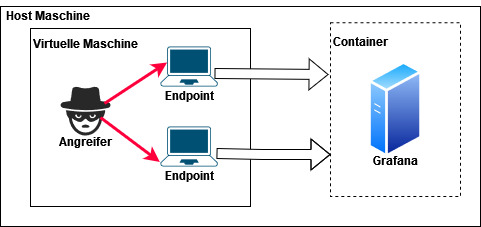
\includegraphics[width=1\textwidth]{assets/Arbeitslabor.jpg}
   \caption[Aufbau unseres Arbeitslabors]
   {Aufbau unseres Arbeitslabors \\Quelle: Eigene Quelle}
   \centering
\end{figure}

Von unserem Aufbau aus streben wir folgende Ziele an: die Aufnahme und Anpassung von Logdateien für Grafana, die Mustererkennung für ausgewählte \glsplural{Cyberangriff} und schließlich die Erstellung von Warnmeldungen für die Endnutzer, damit sie geeignete Sicherheitsmaßnahmen ergreifen können.

\newpage
Der gezielte Ablauf ist in dem folgenden Diagramm dargestellt:

\begin{figure}[H]
   \centering
   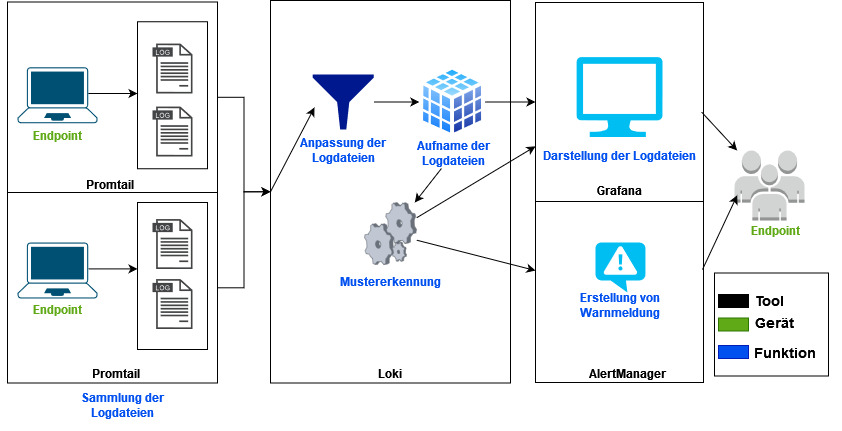
\includegraphics[width=1\textwidth]{assets/Ablauf_grafana2.jpg}
   \caption[Erwarteter Ablauf der Sammlung der Logdateien bis zur Warnmeldung]
   {Erwarteter Ablauf der Sammlung der Logdateien bis zur Warnmeldung \\ Quelle: Eigene Quelle und \citep{Grafana_loki}}
   \centering
\end{figure}

\subsection{Angriffserkennung anhand der Mitre ATT\&CK Matrix}
Es gibt verschiedene Methoden und Frameworks zur Vermeidung, Erkennung und Unterbrechung von \glsplural{Cyberangriff}. Zu den Beispielen gehören das \glsfirst{owasp}, das \glsfirst{CKC}und die \gls{mitre} Matrix, die von \gls{SOC}-Teams verwendet werden, um die Sicherheit von Systemen und/oder Netzwerken zu gewährleisten. Da sich die Richtlinien und Schwerpunkte dieser Frameworks unterscheiden können und somit unterschiedliche Anforderungen an den Aufbau unserer Struktur stellen könnten, haben wir uns entschieden, die \gls{mitre} Matrix zur Erkennung von \glsplural{Cyberangriff} anzuwenden, insbesondere da dieses Framework auch in Splunk integriert ist. Die \gls{mitre} Matrix ist auf \glsfirst{ttp} basiert. Angriffe, Gegenmaßnahmen und Erkennung werden nach \gls{ttp} definiert.

Die \gls{mitre} Matrix hat folgende Hauptnutzung \citep{Mitre_Started}:

{\setstretch{1.5}
\begin{itemize}[noitemsep]
   \item Erkennung und Analyse von Angriffstechnik
   \item	strukturierte Datensammlung über Bedrohungen
   \item	Emulieren von \glsplural{Cyberangriff} für die Anwendung an Angriffsübungen
   \item	Systemhärtung und Verbesserung der Verteidigungsmaßnahmen
\end{itemize}
}

Die Matrix bietet Unternehmen und \gls{SOC}-Teams umfassende Möglichkeiten, um ihre wertvollen Ressourcen zu schützen und ihr Fachwissen im Bereich der \gls{Cybersicherheit} zu erweitern \citep{Hazel_howtousemitre}. In dieser Arbeit konzentrieren wir uns auf die Entwicklung und Implementierung einer Methode zur automatischen Erkennung und Analyse von Angriffstechniken in Grafana.

Das \gls{mitre} Framework besteht aus 14 Taktiken, zu denen jeweils Techniken gehören, die wiederum in Sub-Techniken unterteilt sind. Jede Sub-Technik wird mit Beispielen, Härtungsmaßnahmen und Erkennungsregeln beschrieben.

\begin{figure}[H]
   \centering
   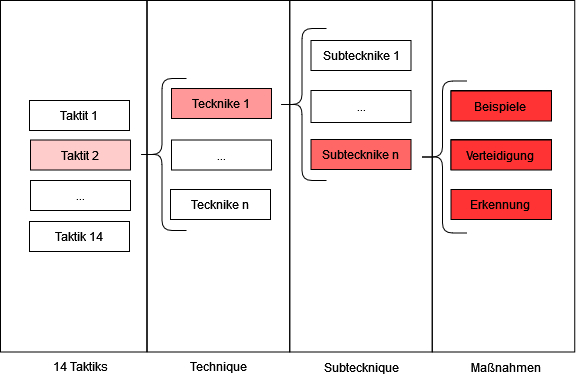
\includegraphics[width=0.8\textwidth]{assets/Mitre_structure.drawio.png}
   \caption[Struktur der \gls{mitre} Matrix]
   {Struktur der \gls{mitre} Matrix \\Quelle: Eigene Quelle und \citep{Mitre_Started}}
   \centering
\end{figure}

{\setstretch{1}
Die 14 Taktiks sind folgende:
\begin{itemize}[noitemsep]
   \item Informationssammlung für zukünftige Angriffe 
   \item	Entwicklung von Ressource von Angreifer
   \item Erster Zugang zum Opfersysteme 
   \item Ausführung von bösartigen Coden
   \item Beharrlichkeit von System
   \item	Privilegienausweitung
   \item Vermeidung von Verteidigungssysteme
   \item \textbf{Zugang zu Anmeldedaten}
   \item Umgebungserkennung
   \item Seitliche Bewegung zu anderem Systemen innerhalb des Angriffsziels
   \item interne Informationssammlung
   \item Steuerung und Kontrolle (C2 - Command and Control im Original)
   \item Datenextrahierung 
   \item	Auswirkung auf die Integrität
\end{itemize}
}

\subsection{Auswahl des Angriffes}
In dieser Arbeit beschäftigen wir uns mit der Taktik \quotes{Zugang zu Anmeldedaten} und deren Technik \gls{bruteforce}. Diese Technik ist in vier Untertechniken aufteilt:

In dieser Arbeit beschäftigen wir uns mit der Taktik \quotes{Zugang zu Anmeldedaten} und ihrer Technik \quotes{\gls{bruteforce}}. Diese Technik ist in vier Untertechniken unterteilt:

{\setstretch{1}
\begin{itemize}[noitemsep]
   \item Erraten von Anmeldedaten 
   \item	Entschlüsselung von \glsplural{hash}
   \item \textit{\gls{stuffing}}
   \item \textit{\gls{spraying}}
\end{itemize}
}

Da unser Ziel hier ist, Grafana zu verwenden, um Angriffe zu erkennen, haben wir uns für einen einfachen und reproduzierbaren Angriff entschieden, der wenige Ressourcen erfordert. In diesem Fall kann ein \gls{bruteforce} mit zwei \glsplural{vm} problemlos durchgeführt werden. Für diesen Angriff verwenden wir die Sub-Technik "Erraten von Anmeldedaten und \textit{\gls{stuffing}}, da sie ähnliche Erkennungsmethoden aufweisen. Andere Maßnahmen schließen wir hierbei aus.

\newpage
Die nächste Abbildung zeigt den Umfang unseres Implementationsversuchs mithifel von \gls{mitre}:
\begin{figure}[H]
   \centering
   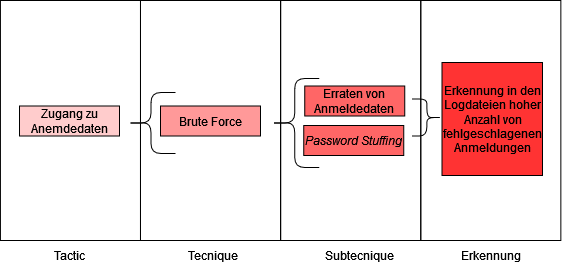
\includegraphics[width=0.7\textwidth]{assets/T1110.drawio.png}
   \caption[\glsfirst{ttp} für unseren Angriff]
   {\glsfirst{ttp} für unseren Angriff \\Quelle: Eigene Quelle und \citep{Mitre_t1110}}
   \centering
\end{figure}

\subsection{Installation und Erstellung von Logdateien}
In diesem Abschnitt konzentrieren wir uns auf die folgenden Punkte:

\begin{enumerate}[noitemsep]
   \item Einrichtung von \glsplural{vm} für das Opfersystem und den Angreifer
   \item Simulation des Angriffe zur Erzeugung von Logdateien
   \item Installation und Konfiguration von Grafana Loki und Promtail mit \gls{container}
   \item Weiterleitung der Logdateien an Grafana
   \end{enumerate}

Die Installation und Verwendung können entweder über die \glsfirst{GUI} oder über die Kommandozeile durchgeführt werden. In dieser Arbeit verwenden wir die Kommandozeile.

\subsubsection{Einrichtung der \glsplural{vm} für Opfersystem und Angreifen}
Die beiden \glsplural{vm} sind eine vorgebaute \quotes{\gls{kali} \glsfirst{vm}} und \quotes{\gls{ubuntu} Server 22.04.2} in ihren standardmäßigen Einstellungen. Beide Maschinen wurden entsprechend ihrer jeweiligen Dokumentation installiert \citep{kali_vm} und \citep{Ubuntu_server}.

\newpage
Für das Opfersystem haben wir uns für die Passwörter \quotes{qwertz} und \quotes{password} entschieden. Laut einer Umfrage gehören diese Passwörter zu den zehn am häufigsten verwendeten Passwörtern in Deutschland \citep{silicon_passwort}.

Für die Durchführung des \gls{spraying} haben wir folgende Passwortkombinationen erstellt:

{\setstretch{1.0}
\begin{lstlisting}[frame=single]
   Opfersystem 1          Opfersystem 2  
   admin:123456           bob:hallo
   user1:passwort         master:alice
   user2:abc123           hans:daniel
   user3:qwertyuiop       bruno:super123
\end{lstlisting}
}

\subsubsection{Generierung von Logdateien mit der Angrifsssimulation}
Für den Angriff verwenden wir folgende Tools:

{\setstretch{1.0}
\begin{itemize}[noitemsep]
   \item	\glsfirst{ssh}
   \item \gls{hydra}
\end{itemize}
}

In diesem Szenario sendet \gls{hydra} gleichzeitig mehrere Authentifizierungsversuche an das Opfersystem, um eine \gls{ssh}-Verbindung herzustellen. Das Tool verwendet ein sogenanntes Wörterbuch mit verschiedenen Einträgen, die als Passwörter dienen. Für unseren Test benutzen wir die bekannte \gls{rockyou}-Datei.

\newpage
Die folgende Abbildung zeigt, wie das \gls{stuffing} abläuft:

\begin{figure}[H]
   \centering
   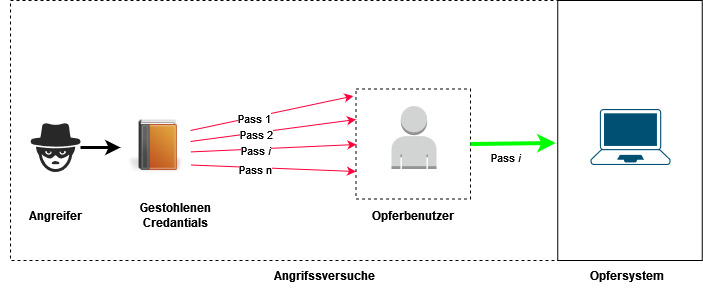
\includegraphics[width=1\textwidth]{assets/Stuffing.jpg}
   \caption[Darstellung von \textit{\gls{stuffing}}]
   {Darstellung von \textit{\gls{stuffing}}\\Quelle: Eigene Quelle und \citep{Nguyen_stuffing}}
   \centering
\end{figure}

\gls{stuffing} wurde mit folgendem Kommando durchgeführt \citep{kali_hydra}:
%Verbatim
{\setstretch{1.0}
\begin{Verbatim}[frame=single]
hydra -l [Benutzername] -P rockyou.txt [Opfersystem] ssh -V -t 4

# Erklärung
-l: Spezifikation des Benutzernamens, den wir angreifen
-P: Auswahl der Datei mit bekannten Passwörtern
ssh: Auswahl der Anwendung, die wir angreifen
-V: Ausführliche Ausgabe über Versuche, Fehler und Erfolg
-t 4: Anzahl von gleichzeitigen Verbindungen
\end{Verbatim}
}

\newpage
Das folgende Bild zeigt einen Teil der Ausgabe von \gls{hydra} während der Ausführung von \gls{stuffing} gegen das Opfersystem1:
\begin{figure}[H]
   \centering
   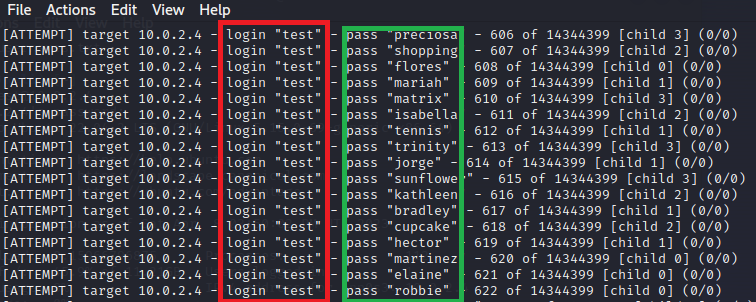
\includegraphics[width=1\textwidth]{assets/stuffing_kali.png}
   \caption[Ausführung von \textit{\gls{stuffing}} gegen Opfersystem1]
   {Ausführung von \textit{\gls{stuffing}} gegen Opfersystem1\\Quelle: Eigene Quelle und \citep{Nguyen_stuffing}}
   \centering
\end{figure}

Und gegen Opfersystem2:
\begin{figure}[H]
   \centering
   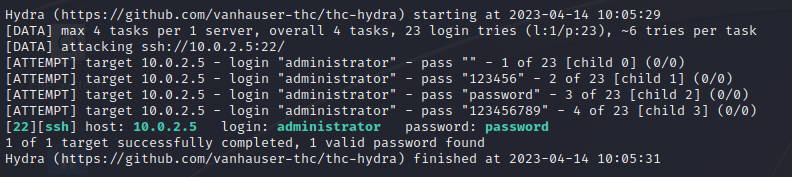
\includegraphics[width=1\textwidth]{assets/stuffing_kali2.png}
   \caption[Ausführung von \textit{\gls{stuffing}} gegen Opfersystem2]
   {Ausführung von \textit{\gls{stuffing}} gegen Opfersystem2\\Quelle: Eigene Quelle und \citep{Nguyen_stuffing}}
   \centering
\end{figure}

\newpage
Unser nächster Angriff, \gls{spraying}, sieht wie folgende aus:
\begin{figure}[H]
   \centering
   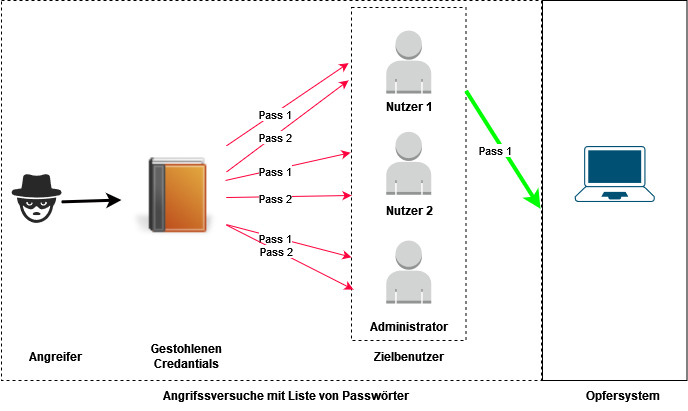
\includegraphics[width=1\textwidth]{assets/Spraying.jpg}
   \caption[Darstellung von \textit{\gls{spraying}}]
   {Darstellung von \textit{\gls{spraying}}\\Quelle: Eigene Quelle und \citep{Swathi_spraxy}}
   \centering
\end{figure}

Für diesen Angriff benutzen wir folgendes Kommando:
{\setstretch{1.0}
\begin{Verbatim}[frame=single]
hydra -L username2.txt -P passwoerter.txt [Opfersystem2] ssh -V -t 4

# Erklärung
-L: Auswahl der Datei mit gefunden Benutzernamen
\end{Verbatim}
}

In diesem Fall gehen wir davon aus, dass der Angreifer einige oder alle Benutzernamen bereits kennt. Da bei diesem Angriff weniger Anmeldeversuche pro Nutzer durchgeführt werden, verwenden wir eine selbst erstellte Datei mit weniger Passwörtern als die \gls{rockyou}-Datei. Unsere Datei enthält die am häufigsten verwendeten Passwörter in Deutschland \citep{silicon_passwort}.

\newpage
Die folgenden Screenshots zeigen die Ausführung von \gls{spraying}:
\begin{figure}[H]
   \centering
   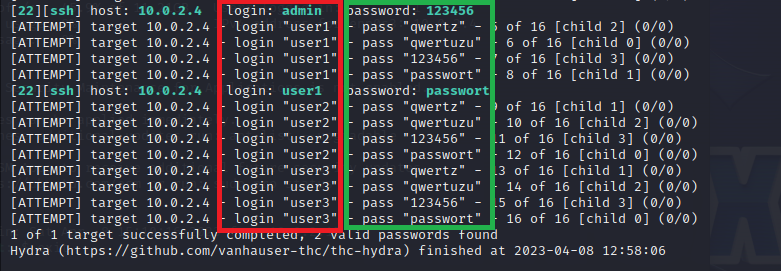
\includegraphics[width=1\textwidth]{assets/Spraying_Kali.png}
   \caption[Ausführung \textit{\gls{spraying}} in Kali Linux gegen Opfersystem1]
   {Ausführung \textit{\gls{spraying}} in Kali Linux gegen Opfersystem1\\Quelle: Eigene Quelle}
   \centering
\end{figure}

\begin{figure}[H]
   \centering
   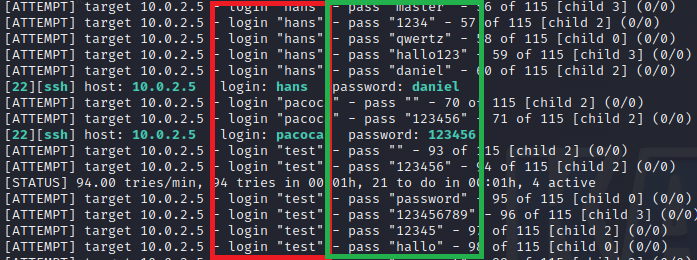
\includegraphics[width=1\textwidth]{assets/Spraying_Kali2.png}
   \caption[Ausführung \textit{\gls{spraying}} in Kali Linux gegen Opfersystem2]
   {Ausführung \textit{\gls{spraying}} in Kali Linux gegen Opfersystem2\\Quelle: Eigene Quelle}
   \centering
\end{figure}

\newpage
\subsubsection{Installation und Einrichtung von Grafana Loki und Promtail}
Die offizielle Dokumentation von Grafana war nicht immer eindeutig in Bezug auf die Ausführung, daher haben wir auch auf externe Quellen zurückgegriffen, um die Einstellungen an unsere Umgebung anzupassen \citep{Polinowski_PGL}. Unter befinden sich die von Grafana zur Verfügung gestellten Konfigurationsdateien und Installationsverfahren \citep{GrafanaLoki_run}:

{\setstretch{1.0}
\begin{lstlisting}[frame=single]
wget https://raw.githubusercontent.com/grafana/loki/v2.8.0/cmd/
loki/loki-local-config.yaml -O loki-config.yaml
(die Datei wurde angepasst)

wget https://raw.githubusercontent.com/grafana/loki/v2.8.0/
clients/cmd/promtail/promtail-docker-config.yaml
-O promtail-config.yaml (die Datei wurde angepasst)

docker-compose -f docker-compose.yaml up 
\end{lstlisting}
}

Im Anhang befinden sich die originalen (Siehe Anhang \ref{appendix:orgGrafana}) und die angepassten Dateien (Siehe Anhang \ref{appendix:AngepasstGrafana}).

Die obigen Kommandos haben folgende Bedeutungen:
\begin{enumerate}[noitemsep]
   \item Herunterladen der Konfigurationsdatei von Loki
   \item Herunterladen der Konfigurationsdatei von Promptail
   \item Ausführung von den \glsplural{container}, indem beide Konfigurationsdateien in eine eingepackt und angepasst wurden und schließlich von der \gls{container}-Anwendung gelesen werden
\end{enumerate}

Für spezifische Versionen oder weitere Einstellungen bietet die Dokumentation umfangreiche Möglichkeiten an \citep{GrafanaLoki_run}.

Für diesen ersten Test wurden die Logdateien des Opfersystems manuell auf den \gls{container} übertragen.

\newpage
\thispagestyle{lscape}
\begin{landscape}
   Nach der Ausführung des Kommandos ist die Anwendung schon benutzbar, wie in dem folgenden Screenshot:
   \begin{center}
      \begin{figure}[H]
         \centering
         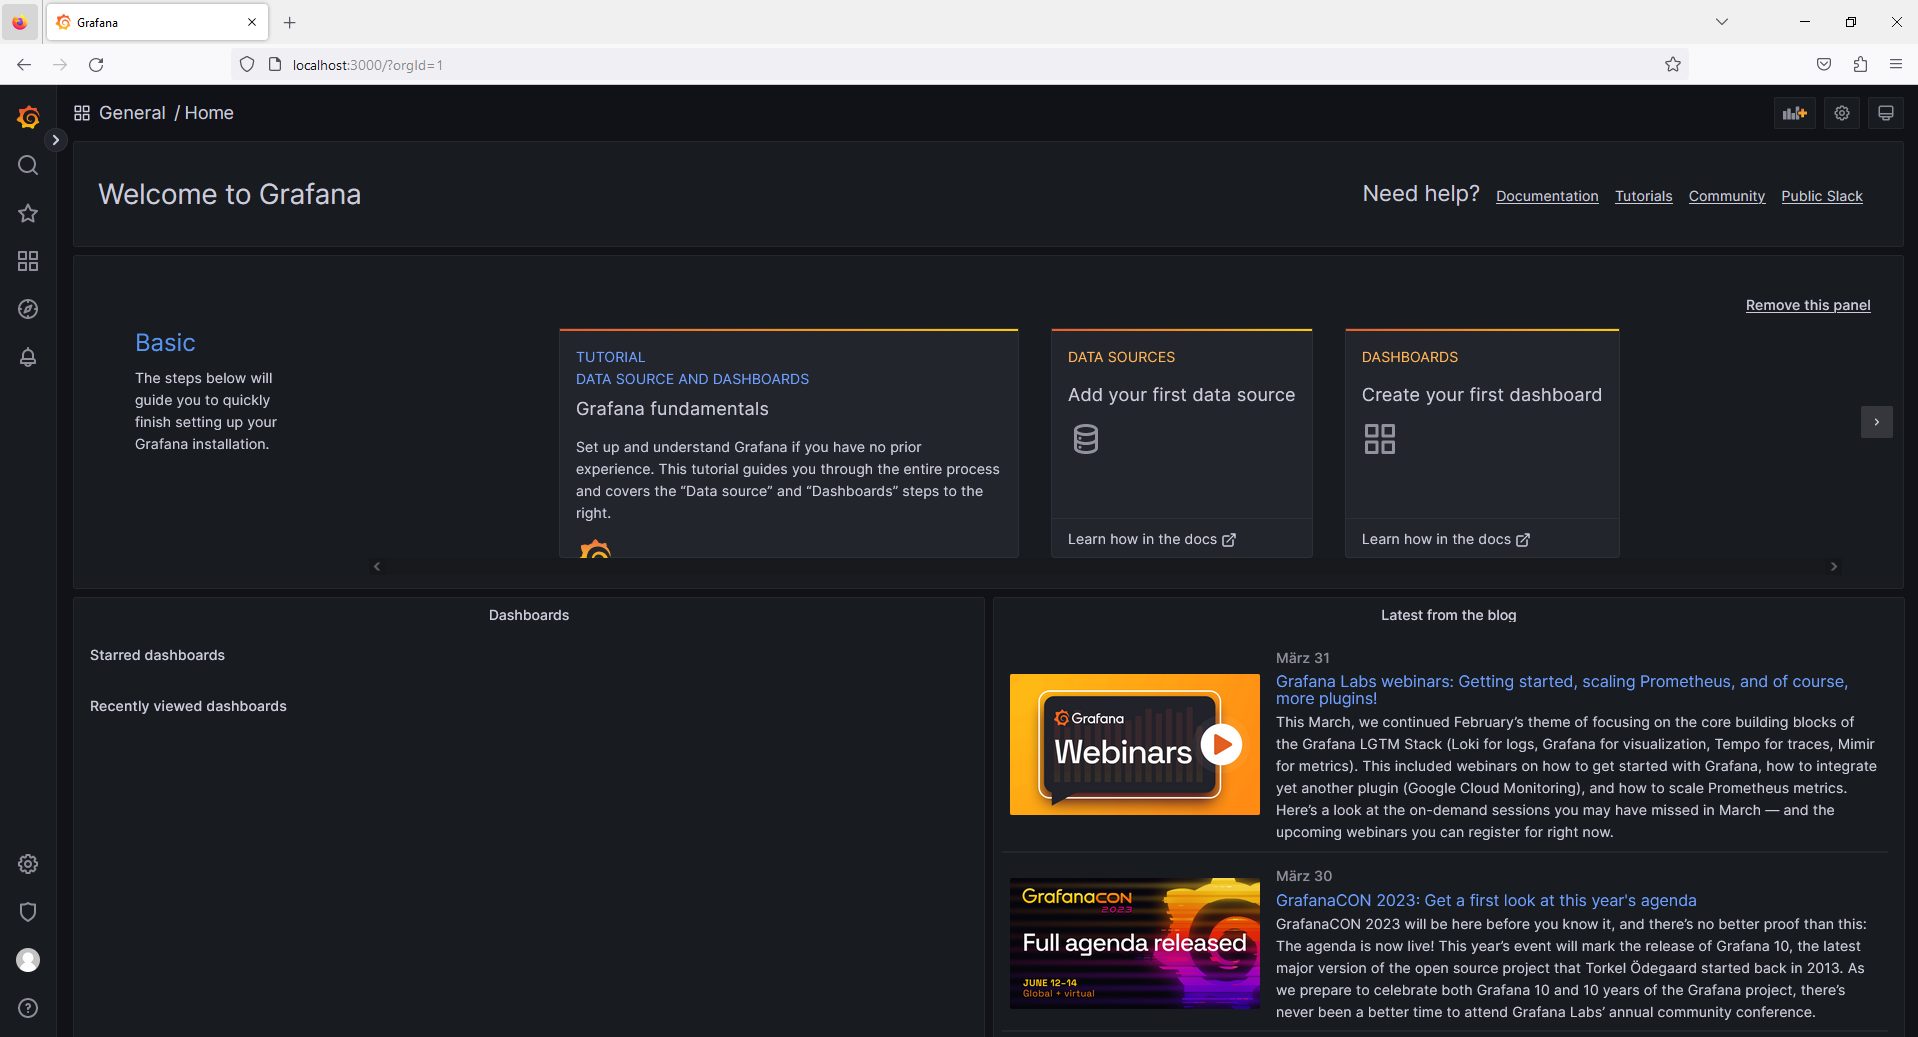
\includegraphics[width=1.3\textwidth]{assets/Installation_Grafana.png}.
         \caption[Screenshot der Willkommensseite von Grafana Loki]
         {Screenshot der Willkommensseite von Grafana Loki\\Quelle: Eigene Quelle und \citep{Grafana_Logs}}
         \centering
      \end{figure}
   \end{center}
\end{landscape}

\subsubsection{Weiterleitung der Logdateien zu Grafana}
Grafana Loki bietet mehrere Möglichkeiten, Logdateien zu empfangen. In unserer Arbeit verwenden wir \textbf{Promtail}, der in einem \gls{container} läuft. Diese Instanz sendet die von uns ausgewählten Logdateien an Grafana und bearbeitet alle Dateien innerhalb eines sogenannten \quotes{jobs}. Wenn wir verschiedene Arten von Logdateien hätten, würde jeder Typ einem eigenen \quotes{job} zugewiesen \citep{Grafana_CollectLogs}. Jeder \quotes{job} hat seine eigenen Regeln, um nach den gewünschten Informationen zu suchen.

In einer produktiven Umgebung wäre die Installation von \textbf{Grafana Agents} auf jedem \gls{Endpoint} eine andere Lösung, um Grafana Loki mit Logdateien zu füllen. In diesem Fall würde jeder \gls{Endpoint} mithilfe von Promtail die Dateien weiterleiten \citep{Grafana_Agents}. Wie bei unserer Lösung müsste der Nutzer für jeden Typ von Logdateien einen spezifischen \quotes{job} konfigurieren.

Der Inhalt von Logdateien lässt sich auch mithilfe der \textbf{\glsfirst{API}} an Grafana Loki senden. In dieser Situation sendet der \gls{Endpoint} eine \gls{http} POST-Anfrage an den Endpunkt von Grafana Loki mit dem Inhalt der Logdateien \citep{Grafana_api}:

{\setstretch{1.0}
\begin{lstlisting}[frame=single][language=json]
# Endpoint 
POST [Addresse_von_Grafana_Loki_Instanz]/loki/api/v1/push

# Inhalt
{
  "streams": [
    {
      "stream": {
        "label": "value"
      },
      "values": [
          [ "Zeit in Unixformat", "<Inhalt der Logdateie>" ],
      ]
    }
  ]
}
\end{lstlisting}
}

Grafana Loki bietet auch eine Integration mit dem Open-Source-Tool OpenTelemetry an, um Logdateien zu empfangen \citep{Grafana_opentelemetry}. Im Allgemeinen wird OpenTelemetry verwendet, um Daten zu senden, zu verarbeiten und zu empfangen. Laut dem Anbieter ist OpenTelemetry mit verschiedenen anderen Tools integriert, um die Datenübertragung zu ermöglichen. Das Tool besteht aus \textit{Agents} und \textit{Collectors}. Der Agent wird auf jedem Endpunkt installiert, um Daten zu sammeln und der Collector empfängt die Daten und leitet sie weiter \citep{Grafana_opentelemetry}. Die Integration mit Grafana Loki erfolgt über die Nutzung von APIs. Der Collector läuft in derselben Umgebung wie Grafana Loki, damit er die Logdateien empfangen und verarbeiten kann. Die \textit{Agents} laufen auf jedem Endpunkt und kommunizieren mit dem \textit{Collector}. Die folgende Abbildung soll diesen Vorgang besser darstellen:

\begin{figure}[H]
   \centering
   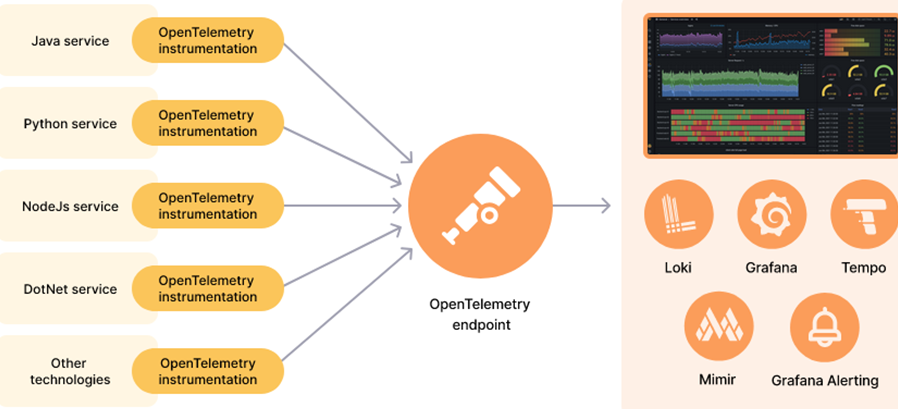
\includegraphics[width=0.8\textwidth]{assets/Grafana_OpenTelemtry.png}
   \caption[Datenfluss zwischen OpenTelemetry und Grafana Loki]
   {Datenfluss zwischen OpenTelemetry und Grafana Loki\\Quelle: \citep{Grafana_WhatOpentelemetry}}
   \centering
\end{figure}

An der linken Seite haben wir die verschiedenen \glsplural{Endpoint}, auf denen jeweils ein \textit{Agent} läuft. In der Mitte haben wir den \textit{Collector}, der die Logdateien schließlich an Grafana Loki und/oder an andere Tools weiterleitet.

\newpage
\subsection{Aufbau der Erkennungsregel für den ausgewählten Angriff}
Ein \gls{bruteforce} lässt sich durch die Anzahl der fehlgeschlagenen Anmeldeversuche erkennen \citep{Selvaganesh_SplunkBruteForce}. Wir betrachten eine Situation, in der keine Gegenmaßnahmen wie Kontosperre nach \textit{n} beliebigen Versuchen oder \gls{mfa}, implementiert sind. Das folgende Aktivitätsdiagramm stellt einen allgemeinen Ablauf eines Anmeldungsverfahrens dar

\begin{figure}[H]
   \centering
   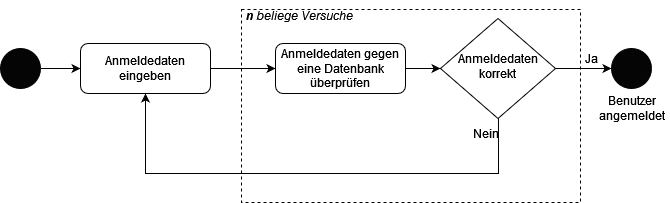
\includegraphics[width=0.8\textwidth]{assets/Anmeldeverfahren.drawio.png}
   \caption[Allgemeiner Ablauf eines Anmeldungsverfahrens]
   {Allgemeiner Ablauf eines Anmeldungsverfahrens \\Quelle: Eigene Quelle und \citep{Selvaganesh_SplunkBruteForce}}
   \centering
\end{figure}

Grafana Loki bietet ein Konfigurationsmuster für die Eingabe und Darstellung von \gls{ssh} Logdateien an. In dieser Konfiguration sind bereits Grafiken und Regelsets enthalten, die eine umfassende Analyse dieser Daten ermöglichen \citep{VoidQuark_sshlogs}. Die extrahierten Logdateien werden mithilfe der folgenden Elemente gelesen und bearbeitet:

\begin{table}[H]
   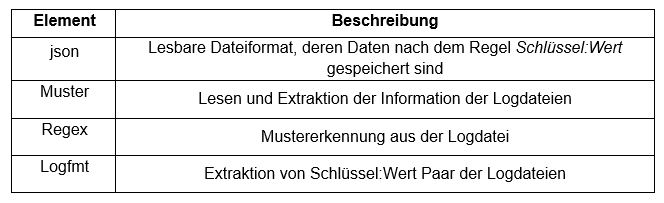
\includegraphics[width=\linewidth]{assets/tabelle_sshgrafana.png}
   \caption[Elementen eines Regelsätzes in Grafana Loki]
   {Elementen eines Regelsätzes in Grafana Loki \\Quelle: Eigene Quelle, \citep{VoidQuark_sshlogs} und \citep{Setter_Logfmt}}
\end{table}



% \begin{table}[]
%    \begin{tabular}{|c|c|}
%    \hline
%    sum by(add) (rate({job=\quotes{varlogs}, instance=~\quotes{\$instance}} & Hiermit wird die Aufsummierung der Benutzernamen definiert, die wir mit \quotes{Patterns} in LogQL definiert haben. \quotes{Patterns} ermöglichen die einfache Extrahierung von Informationen aus einer Zeile. Wir holen alle Log-Einträge, die sich auf den Job \quotes{varlogs} beziehen. Wir können auch nach spezifischen Endpoint filtern, indem wir das Schlüsselwort \quotes{instance} benutzen. \\ \hline

%    | &  \\ \hline

%    |= `\textbf{\textcolor{red}{sshd}}[` \\ |= `: \textbf{\textcolor{red}{Failed}}` & \quotes{|} funktioniert in LogQL wie eine Pipeline für die Verkettung von mehreren Suchmustern. \\ \hline

%    !~ `invalid user` \\ !~ `test` !~ `10.0.2.15` & Regular Expression für die Suche nach Zeilen \textbf{ohne} diese Einträge. Wir können beispielsweise Einträge ausschließen, die sich nicht bösartige Nutzer sind, um falsche Positive zu vermeiden \\ \hline

%    | pattern `<_> for <\textbf{\textcolor{blue}{Benutzername}}> from \<\textbf{\textcolor{blue}{QuelleAddress}}\> port <_>` [\$__range])) &  Die Definition der Wörter \quotes{Benutzername} \quote{QuelleAddress} und als \quote{Pattern} dienen dazu, einen Benutzernamen und eine Quelle IP-Adresse aus der Logdatei zu extrahieren. Die Platzhalter \quote{<_>}sind unbenannte Elemente, die in diesem Fall auf die Einträge  \quote{“password”} und Portnummber in der Zeile verweisen.\\ \hline
%    \end{tabular}
% \end{table}

%https://grafana.com/docs/loki/latest/fundamentals/labels/
%https://prometheus.io/docs/concepts/jobs_instances/

Für jedes Angriffszenario benutzen wir spezifische Regeln, die mit \gls{logql} aufgebaut sind. Die Filterung findet mithilfe von zweil Labels \quotes{Instance} und \quotes{Job} statt. In Promtail wird jeder \gls{Endpoint} als \quotes{Instance} bezeichnet. Eine oder mehrere \quotes{Instances} werden einem \quotes{Job} zugewiesen. \quotes{Jobs} beziehen sich auf die Bearbeitung der Logdateien nach dem spezifizieren Regeln, in unserem Fall, Überprüfung von \gls{ssh}-Logdateien. Diese Struktur stammt aus dem Tool \gls{prometheus}. Alle unsere \quotes{Instance} werden in einem \quotes{Job} eingepackt, wo sie nach den gleichen Regeln verarbeitet. Das folgende Diagramm stellt die Beziehung zwischen dieser beiden Labels dar:

\begin{figure}[H]
   \centering
   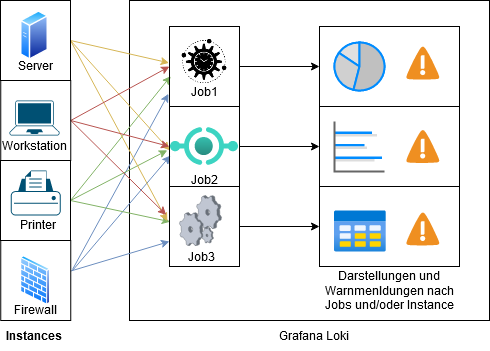
\includegraphics[width=0.8\textwidth]{assets/Instance_Jobs.drawio.png}
   \caption[Beziehung zwischen \quotes{Instance} und \quotes{Job}]
   {Beziehung zwischen \quotes{Instance} und \quotes{Job} \\Quelle: Eigene Quelle und \citep{Prometheus_JobInstance}}
   \centering
\end{figure}


In dem nächsten Abschnitt beschreiben wir, wie diese Regel in \gls{logql} geschrieben werden.

\newpage
\subsubsection{Regelsätze in LogQL}
In diesem Abschnitt fassen wir zusammen, wie eine Abfrage in \gls{logql} für eine Logdatei mit \gls{ssh} Einträge aussieht. Für ausführliche Informationen über den Aufbau der Abfrage empfehlen wir die offizielle Dokumentation, auf die diese Erklärung basiert ist \citep{Grafana_logql}. Unsere Logdatei enthält unter anderem folgende Zeile:

{\setstretch{1.0}
\begin{Verbatim}[frame=single]
14 14:05:30 opfersystem2 sshd[1698]: Failed password for administrator 
from 10.0.2.15 port 58036 ssh2
\end{Verbatim}
}

Um \gls{ssh}-Einträge zu erkennen und bestimmte Informationen zu extrahieren, die anzeigen, ob es sich um einen fehlgeschlagenen Anmeldeversuch handelt, extrahieren und später summieren wir die hervorgehobenen Elemente auf:

{\setstretch{1.0}
\begin{Verbatim}[commandchars=\\\{\},frame=single]
14 14:05:30 opfersystem2 \textbf{\textcolor{red}{sshd[}}1698]: \textbf{\textcolor{red}{Failed}} password for \textbf{\textcolor{blue}{administrator}}
from \textbf{\textcolor{blue}{10.0.2.15}} port 58036 ssh2
\end{Verbatim}
}

Wir teilen die Abfrage unten mit, um ihre Bestandteile besser zu verstehen: 
\begin{table}[H]
   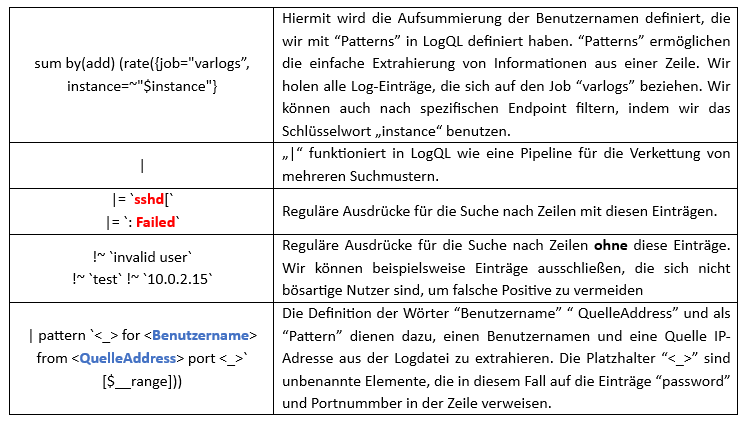
\includegraphics[width=1\linewidth]{assets/tabelle_logql.png}
   \caption[Aufbau der Regelsätze in Grafana Loki für \gls{ssh} Logdateien]
   {Aufbau der Regelsätze in Grafana Loki für \gls{ssh} Logdateien \\Quelle: Eigene Quelle, \citep{VoidQuark_sshlogs} und \citep{Grafana_logql}}
\end{table}

% \begin{table}[]
%    \begin{tabular}{|c|X|}
%    \hline
%    % sum by(add) (rate({job=\quotes{varlogs},\\ instance=~\quotes{\$instance}} & Hiermit wird die Aufsummierung der Benutzernamen definiert, die wir mit \quotes{Patterns} in LogQL definiert haben. \quotes{Patterns} ermöglichen die einfache Extrahierung von Informationen aus einer Zeile. Wir holen alle Log-Einträge, die sich auf den Job \quotes{varlogs} beziehen. Wir können auch nach spezifischen Endpoint filtern, indem wir das Schlüsselwort \quotes{instance} benutzen. \\ \hline

%    | &  \\ \hline

%    |= `\textbf{\textcolor{red}{sshd}}[` \\ |= `: \textbf{\textcolor{red}{Failed}}` & \quotes{|} funktioniert in LogQL wie eine Pipeline für die Verkettung von mehreren Suchmustern. \\ \hline

%    !~ `invalid user` \\ !~ `test` !~ `10.0.2.15` & Regular Expression für die Suche nach Zeilen \textbf{ohne} diese Einträge. Wir können beispielsweise Einträge ausschließen, die sich nicht bösartige Nutzer sind, um falsche Positive zu vermeiden \\ \hline

%   % | pattern `<_> for <\textbf{\textcolor{blue}{Benutzername}}> from \<\textbf{\textcolor{blue}{QuelleAddress}}\> port <_>` [\$__range])) &  Die Definition der Wörter \quotes{Benutzername} \quote{QuelleAddress} und als \quote{Pattern} dienen dazu, einen Benutzernamen und eine Quelle IP-Adresse aus der Logdatei zu extrahieren. Die Platzhalter \quote{<_>}sind unbenannte Elemente, die in diesem Fall auf die Einträge  \quote{“password”} und Portnummber in der Zeile verweisen.\\ \hline
%    \end{tabular}
% \end{table}



\textbf{\textcolor{red}{Das sollte verbessert werden}}
Eine Erkennungsregel hätte folgende Logik:
{\setstretch{1.0}
\begin{Verbatim}[frame=single]
   # Gefundene Werte in den Logdateien
   # Av = Anzahl fehlgeschlagener Anmeldungsversuche
   # Ia = Intervallzeit zwischen fehlgeschlagenen Anmeldungsversuchen

   # Festgelegte Werte für legitime und bösartige Verbindungen
   # Ga = Grenze zwischen legitimen und bösartigen Anmeldungsversuchen
   # Nt = Intervallzeit zwischen legitimen Anmeldungsversuchen

   wenn (Av >= Ga) und (Ia < Nt)
      Warnmeldung(Brutefoce)
   sonst
      weiterBeobachten()
\end{Verbatim}
}




\subsection{Hinzufügen der Regelsätze Grafana Loki}

Die Regelsätze in Grafana Loki können sowohl manuell im Menü \quotes{Code} als auch über die \gls{GUI} im Menü \quotes{Builder} geschrieben werden. Letzteres bietet eine benutzerfreundlichere Umgebung, um die Regeln zu schreiben. Die folgenden Abbildungen zeigen diese beiden Optionen:

\begin{figure}[H]
   \centering
   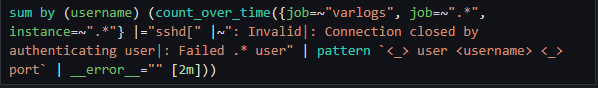
\includegraphics[width=1\textwidth]{assets/manuellerCodeLoki.png}
   \caption[\quotes{Code} in Grafana Loki für manuelle die Eingabe des \gls{logql}-Codes]
   {\quotes{Code} in Grafana Loki für manuelle die Eingabe des \gls{logql}-Codes. \\ Quelle: \citep{VoidQuark_sshlogs}}
   \centering
\end{figure}

\begin{figure}[H]
   \centering
   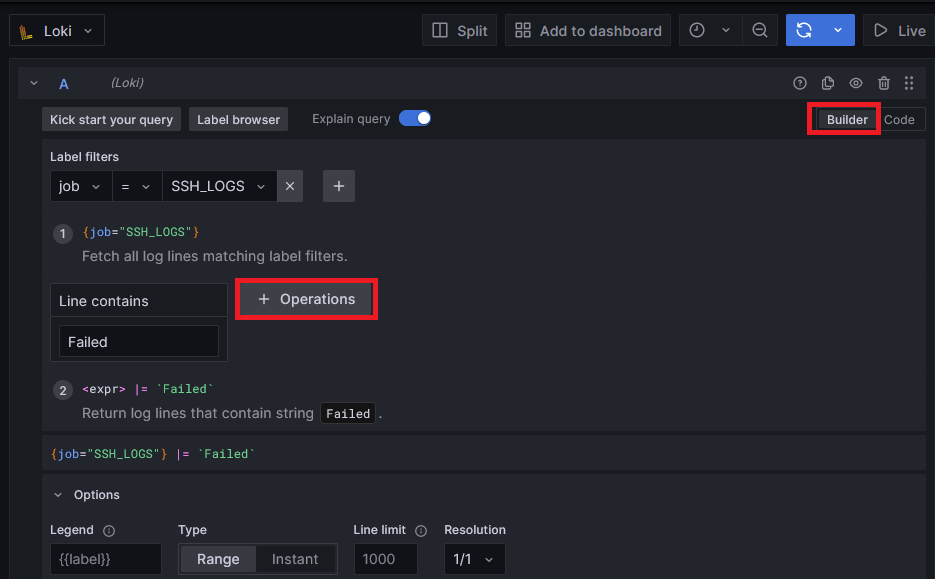
\includegraphics[width=1\textwidth]{assets/klickibuntyGrafana.png}
   \caption[\quotes{Builder} in Grafana Loki für nutzerfreundlichere Eingabe des \gls{logql}-Codes.]
   {\quotes{Builder} in Grafana Loki für nutzerfreundlichere Eingabe des \gls{logql}-Codes. Quelle: \citep{VoidQuark_sshlogs}}
   \centering
\end{figure}

Beide Optionen bieten die Möglichkeit, eine Erklärung zur Abfrage anzuzeigen:
\begin{figure}[H]
   \centering
   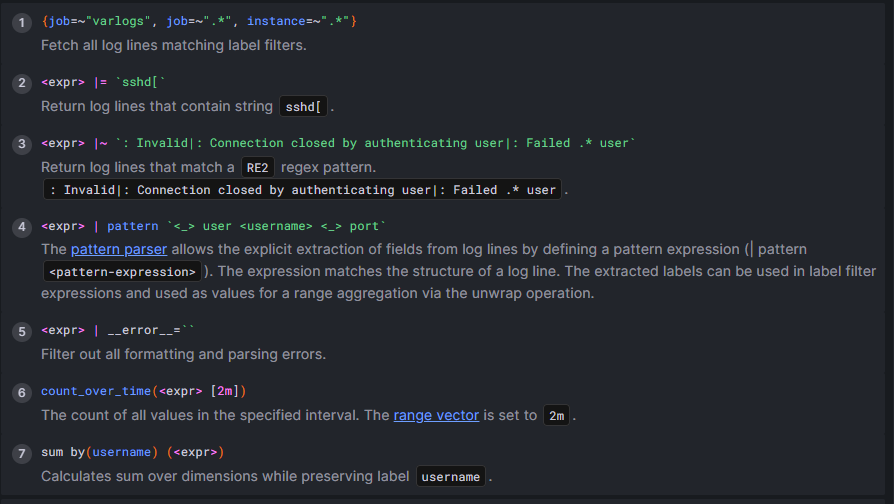
\includegraphics[width=1\textwidth]{assets/erklaerungLoki.png}
   \caption[Ausführliche Information über die Abfrage]
   {Ausführliche Information über die Abfrage\\Quelle: \citep{Grafana_QueryEditor}}
   \centering
\end{figure}

\newpage
\thispagestyle{lscape}
\begin{landscape}
   Nachdem die \gls{ssh}-Logdateien gelesen und bearbeiten wurden, bekommen wir von Grafana Loki folgende Zasammenfasung der Ergebnissen:
   \begin{center}
      \begin{figure}[H]
         \centering
         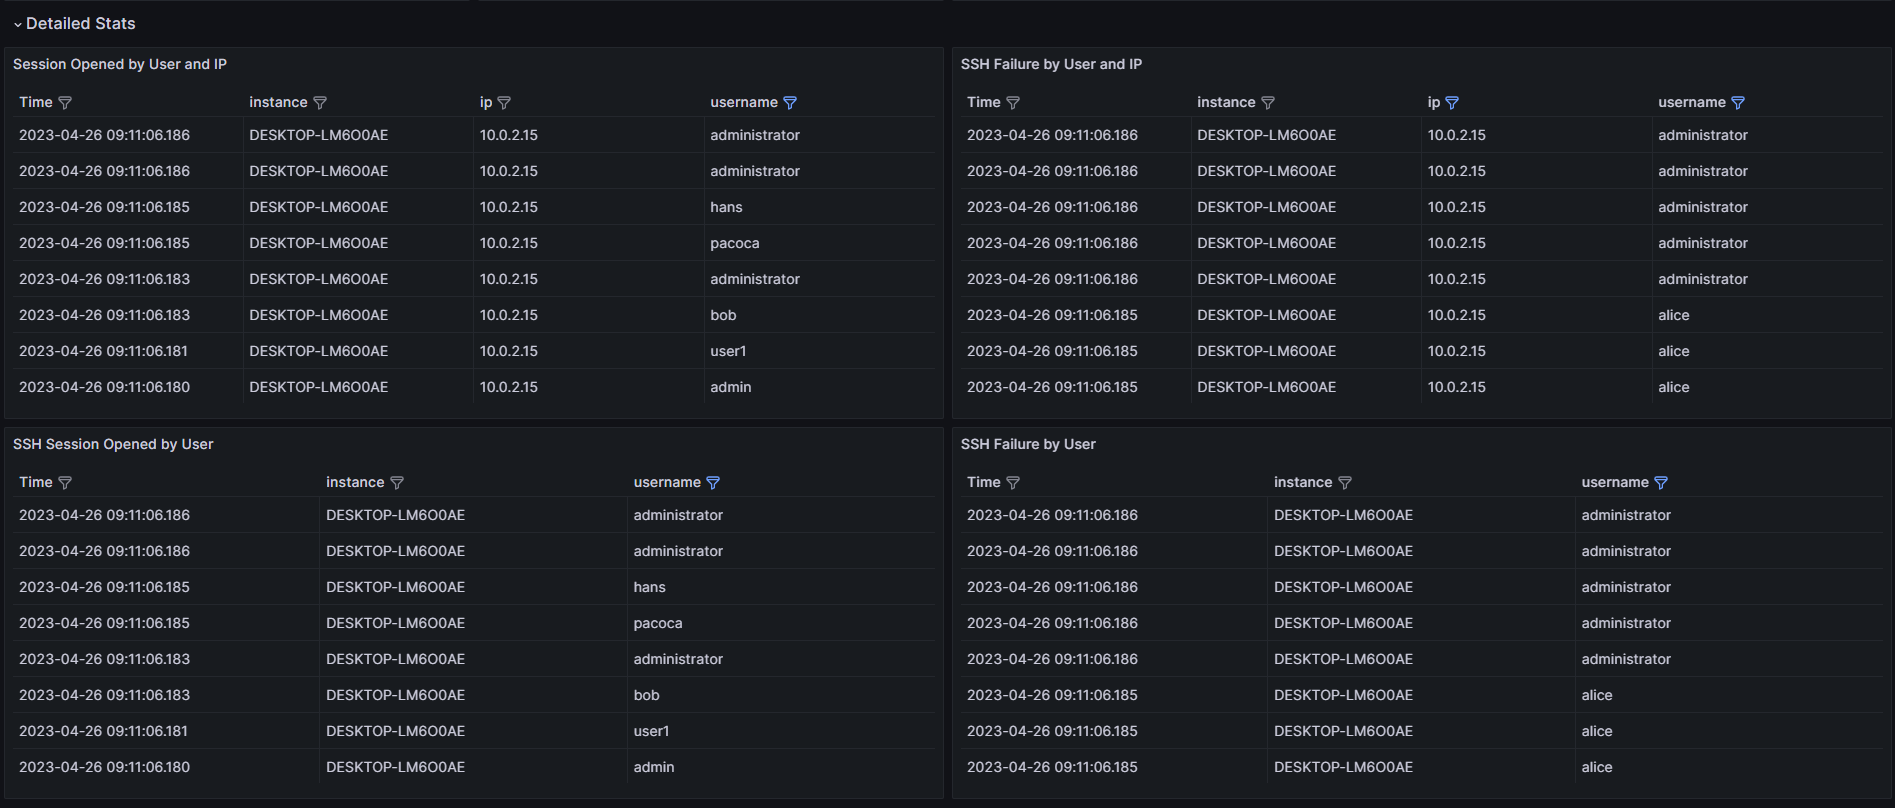
\includegraphics[width=1.3\textwidth]{assets/GrafanaLoki_sshDetailed.png}.
         \caption[Bearbeitung der \gls{ssh} Logdateien von Grafana Loki]
         {Bearbeitung der \gls{ssh} Logdateien von Grafana Loki\\Quelle: Eigene Quelle and \citep{VoidQuark_sshlogs}}
         \centering
      \end{figure}
   \end{center}
\end{landscape}

\newpage
\thispagestyle{lscape}
\begin{landscape}
   Das nächste Bild gibt ausführliche Informationen der Logdateien:
   \textbf{Bild Korrigieren}
   \begin{center}
      \begin{figure}[H]
         \centering
         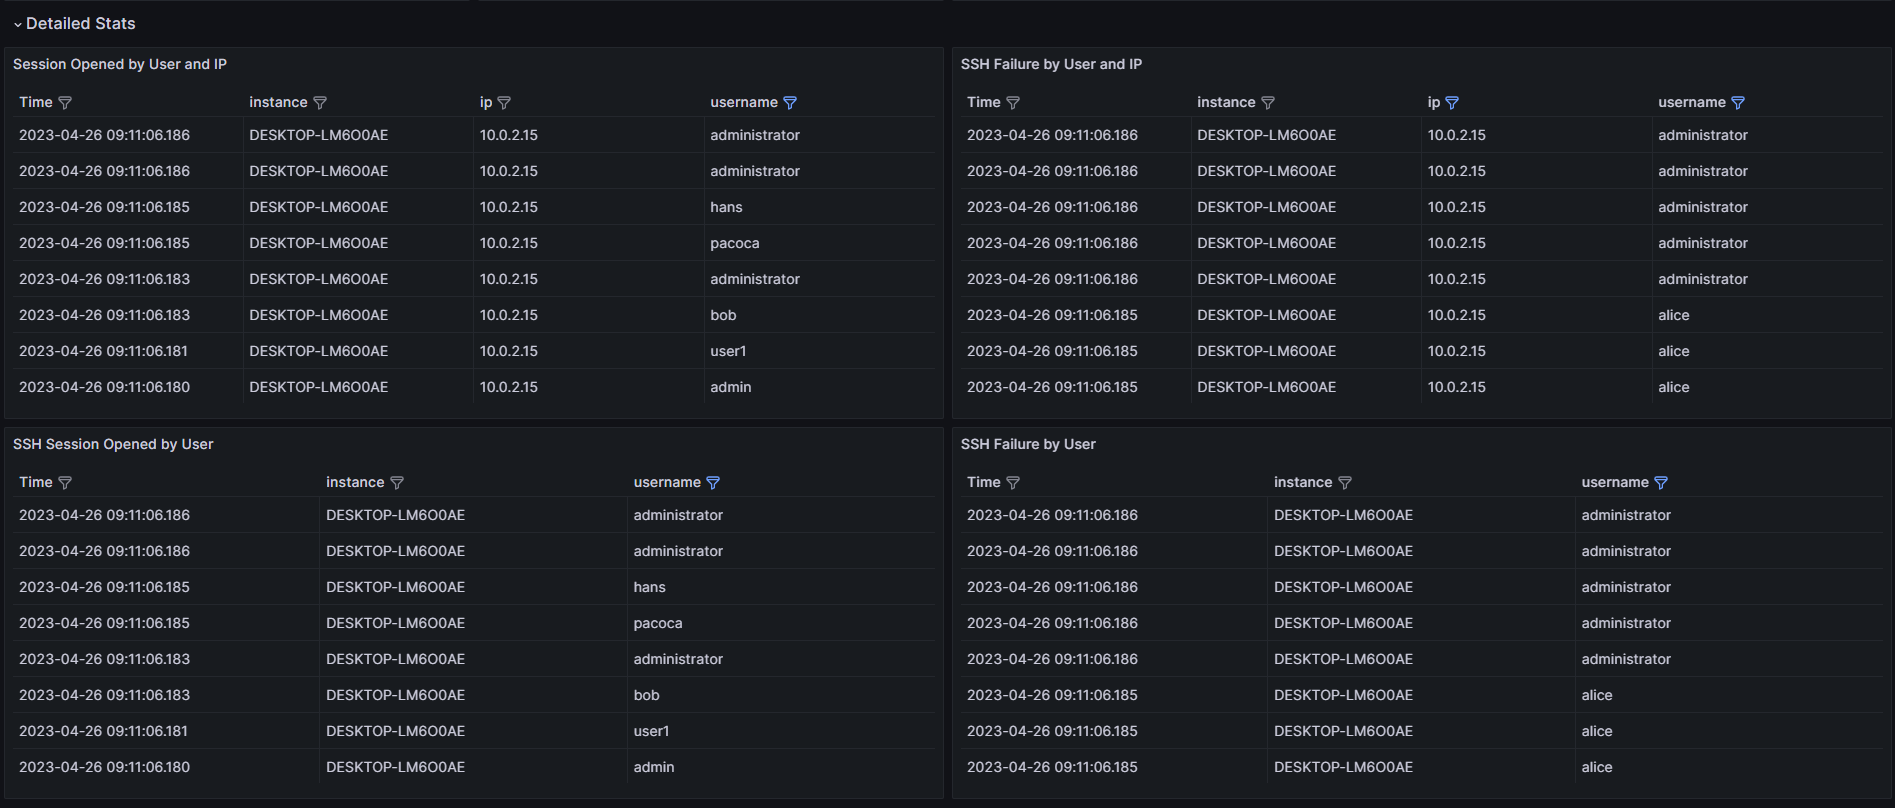
\includegraphics[width=1.3\textwidth]{assets/GrafanaLoki_sshDetailed.png}.
         \caption[Ausführliche Darstellung der \gls{ssh} Logdateien von Grafana Loki]
         {Ausführliche Darstellung der \gls{ssh} Logdateien von Grafana Loki\\Quelle: Eigene Quelle and \citep{VoidQuark_sshlogs}}
         \centering
      \end{figure}
   \end{center}
\end{landscape}

\subsection{Einrichtung des Warnmeldungskomponent}
In den vorherigen Teilen dieser Arbeit haben wir uns damit auseinandergesetzt, Grafana so einzustellen, dass wir schließlich eine Lösung ähnlich einer \gls{SIEM} erhalten. Von unseren ursprünglichen Vorschlägen haben wir bereits Folgendes erreicht:

{\setstretch{1}
\begin{enumerate}[noitemsep]
   \item	Sammlung der Logdateien aus den \glsplural{Endpoint} mit Promtail
   \item Anpassung der Logdateien für die nachträgliche visuelle Darstellung mit Loki
   \item Nutzung von Regelsätzen in Loki für die Analysierung der \gls{ssh} Logdateien
   \item Graphische Darstellung der Logdateien in Grafana mit den in Loki verwendeten Regelsätzen
\end{enumerate}
}
Unser letztes Ziel besteht darin, Warnmeldungen für potenzielle Angriffe mithilfe der Ergebnisse von Loki zu generieren. Grafana kann intern und extern mit Tools integriert werden, um Warnmeldungen zu erstellen. Eines dieser externen Tools ist der \textbf{Alertmanager}, der bereits integriert ist. Dieses Tool kann Daten von \gls{prometheus}, \gls{cortex} und \gls{mimir} als Datenquelle verwenden \citep{Grafana_Alertmanager} und kann Daten von beliebigen \glsplural{Endpoint} empfangen. Die Regelsätze des Alertmanagers haben folgendes Muster:

{\setstretch{1.0}
\begin{Verbatim}[frame=single]
# Warnmeldungen können in beliebigen Gruppen kategorisiert werden. Diese
können von den Nutzern entsprechend ihrer Anforderungen und Bedürfnisse 
definiert werden.
groups:

      # Ab diesem Punkt beginnen wir mit der Definition der Regelsätze 
      für die Erkennung von Warnmeldungen. Diese umfassen:
   - name: example
     rules:
    - alert: HighRequestLatency

      # LogQL-Regelsätze für die Erkennung der Warnmeldung, welche die 
      in den vorherigen Schritten definierten Abfragen verwenden.
      expr: job:request_latency_seconds:mean5m{job="myjob"} > 0.5
      for: 10m
       labels:
         severity: page
       annotations:
         summary: High request latency
\end{Verbatim}
}

%verbatim comments
%lst listing

Grafana hat auch ein eigenes internes Tool, um Warnmeldungen zu konfigurieren: \textbf{Alerting}. In dieser Arbeit versuchen wir unser Warnmeldungs-System mithilfe dieses Tools aufzubauen.

Die Warnmeldungen können direkt in der \gls{GUI} von Grafana konfiguriert werden. Dazu folgt man den folgenden Schritten \citep{Grafana_alerting}:

{\setstretch{1}
\begin{enumerate}[noitemsep]
   \item Name der Regel
   \item Regelsätze in \gls{logql}
   \item Definition von Gruppen für jede Art von Warnmeldung. Gruppen können später verschiedenen Einstellungen zugewiesen werden, wie z.B. Benachrichtigungen und Inhalte.
   \item Informationen über die Warnmeldung, wie eine eindeutige ID und eine Beschreibung. Der Nutzer kann diese Felder so definieren, wie es notwendig ist.
   \item Benachrichtigung der Zielgruppe, die diesen Fall später bearbeiten wird.
   \item Labels zur besseren Organisation der Warnmeldungen.
   \item Konfiguration von E-Mail in Grafana für die Weiterleitung der Warnmeldungen.
\end{enumerate}
}

Für unseren ersten Test erstellen wir Warnmeldungen für fehlgeschlagene Anmeldeversuche. Wir haben die oben genannten Elemente definiert und die folgenden Regelsätze verwendet \citep{VoidQuark_sshlogs}:

{\setstretch{1.0}
\begin{Verbatim}[frame=single]
# (A) Anzahl von fehlgeschlagenen Anmeldeversuche für existierenden
Benutzernamen:
sum by (username) (count_over_time({$label_name=~"$label_value", 
job=~"$job", instance=~"$instance"} |="sshd[" |~": Invalid|: 
Connection closed by authenticating user|: Failed .* user" | 
pattern `<_> user <username> <_> port` | __error__="" 
[$__interval]))

# (B) Anzahl von Fehlgeschlagenen Anmeldeversuche für nicht 
existierenden Benutzernamen:
sum by (username) (count_over_time({$label_name=~"$label_value", 
job=~"$job", instance=~"$instance"} |="sshd[" |=": Failed" !~"invalid 
user" | pattern `<_> for <username> from <_> port` | __error__=""
[$__interval]))

# Wenn die Anzahl von (A) oder von (B) größer als fünf ist, dann wird
die Warnmeldung als E-Mail an dem Ziel geschickt.
\end{Verbatim}
}

% discard lines with Server Ansible - https://grafana.com/docs/loki/latest/logql/log_queries/

Im Anhang (Siehe Anhang \ref{appendix:Warnmedungskonfiguration}) befindet sich die Konfigurationsdatei für unsere Warnmeldung. Nachdem alles korrekt konfiguriert wurde, haben wir die folgende E-Mail erhalten:

\begin{figure}[H]
   \centering
   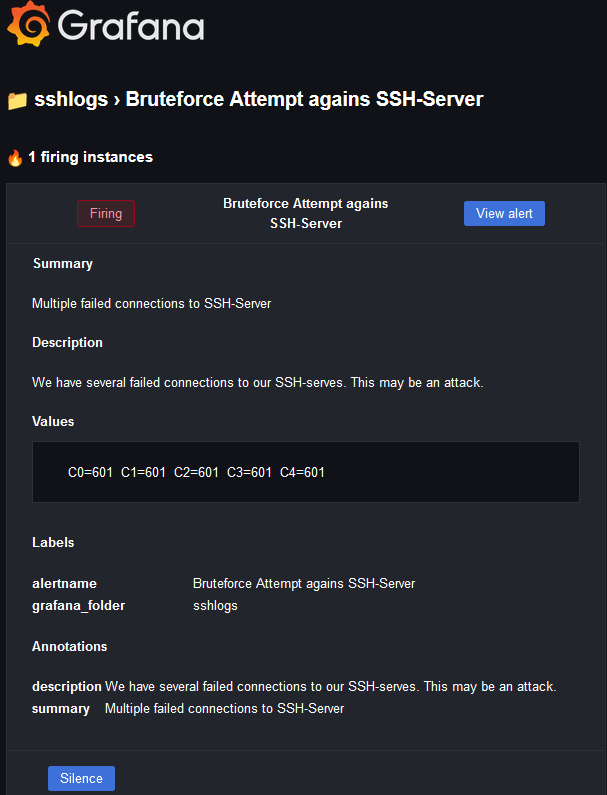
\includegraphics[width=0.7\textwidth]{assets/GrafanaWarnmeldung.png}
   \caption[E-Mail Warnmeldung von Grafana]
   {E-Mail Warnmeldung von Grafana \\Quelle: Eigene Quelle und \citep{Grafana_alerting}}
   \centering
\end{figure}

Das Alerting-Tool von Grafana bietet keine direkte Integration zu einem \gls{IDS}, \gls{IPS}, \gls{SIEM} oder einer \gls{API} an. Die Kommunikation mit solchen \glsplural{Endpoint} lässt sich jedoch mithilfe von \textbf{\gls{webhook}} konfigurieren \citep{Grafana_Notifications}.

% enabled = true
% host = smtp.gmail.com:587
% user = alertsgrafanaBA@gmail.com
% # If the password contains # or ; you have to wrap it with triple quotes. Ex """#password;"""
% password = "sexpjkbdsdwrkgqm"